% ==============================================================================
% Section 3.2: In-Corpus Visual Document RAG - ColPali vs VisRAG
% Owner: Member 2 (TV2) | Target length: ~5.5-6.5 pages
% ==============================================================================

\section{Tầng In-Corpus Visual Document RAG: Đối chứng ColPali và VisRAG}
\label{sec:method_vision_doc}


Sau khi chọn kho, hệ thống phải tìm trang có thông tin để trả lời.
ColPali và VisRAG đều tìm trực tiếp trên ảnh trang. ColPali lưu nhiều
vector mỗi trang để từng token truy vấn có thể khớp với một vùng ảnh.
VisRAG-Ret lưu một vector cho mỗi trang, còn VisRAG-Gen đọc các ảnh đã
truy xuất để tạo câu trả lời \cite{faysse2025colpali,yu2025visrag}.
Ở bước retrieval, ta kiểm tra trang đúng đứng ở đâu. Ở bước generation,
ta kiểm tra mô hình có đọc đúng thông tin từ trang đó hay không.

\subsection{Page-as-Image trong truy xuất tài liệu PDF}
\label{subsec:vision_paradigm}

Trong tài liệu PDF, bố cục giúp người đọc hiểu ý nghĩa của số liệu.
Một ô trong bảng cần được đọc cùng tiêu đề hàng, tiêu đề cột và đơn vị.
Với biểu đồ, nhãn trục và chú giải cho biết số liệu thuộc thời điểm
hoặc nhóm nào. Với Page-as-Image, ColPali và VisRAG dùng ảnh của cả
trang PDF làm đầu vào cho bộ mã hóa và giữ bố cục trong ảnh. Khi có
câu hỏi, bộ truy xuất xếp hạng các trang theo mức độ liên quan
\cite{faysse2025colpali,yu2025visrag}.

\subsubsection{Ví dụ đọc thông tin từ bảng và biểu đồ trong PDF}

Giả sử một biểu đồ trong báo cáo cho thấy doanh thu quý 3 là 80 tỷ
đồng và doanh thu quý 4 là 100 tỷ đồng. Nhãn dưới mỗi cột cho biết số
liệu thuộc quý nào. Lấy doanh thu quý 3 làm mốc so sánh, ta có
\[
    \frac{100-80}{80}\times100\% = 25\%.
\]
Văn bản trích xuất có thể chứa cả hai con số nhưng thiếu thông tin
cho biết số nào thuộc quý nào. Khi đó hệ thống dễ lấy nhầm mốc so
sánh. Với bảng, đọc đúng một con số vẫn chưa đủ. Nó phải đi cùng
đúng hàng, cột và đơn vị.

Một cấu hình TextRAG có thể phân tích bố cục trang (layout parsing),
dùng OCR để nhận dạng ký tự và tạo mô tả cho hình ảnh (captioning).
Sau đó, hệ thống chia văn bản thành các đoạn (chunks) để lập chỉ mục. Một cách xếp hạng
trang là lấy điểm của đoạn khớp nhất trong trang đó. ColPali tính
MaxSim ở mức token truy vấn, như trình bày ở
Mục~\ref{subsec:colpali} \cite{faysse2025colpali}.

Truy xuất bằng ảnh trang giúp giữ vị trí của giá trị, nhãn và chú thích. Khả năng đọc các chi tiết này vẫn phụ thuộc vào độ phân giải và chất lượng bản quét. Trang có chữ nhỏ có thể mất chi tiết khi bị thu nhỏ. Với PDF có lớp văn bản rõ và câu hỏi cần tìm đúng một mã tài liệu, tìm kiếm theo từ khóa vẫn là một đối chứng phù hợp.

Khi đánh giá hệ thống, cần kiểm tra hai bước. Ở bước truy xuất, ta xem top-$k$ có chứa trang cần thiết hay không. Ở bước tạo câu trả lời, ta xem mô hình có đọc và diễn giải đúng thông tin trên các trang nhận được hay không. Cách kiểm tra này được dùng để phân tích kết quả của VisRAG ở Chương~\ref{chap:experiments}.

\subsection{ColPali với Multi-vector Embeddings và Late Interaction}
\label{subsec:colpali}

\subsubsection{Kiến trúc mô hình và luồng xử lý}

ColPali mở rộng PaliGemma-3B bằng một lớp chiếu đưa đầu ra của mỗi token
về không gian 128 chiều. Khi lập chỉ mục, mô hình lưu nhiều vector cho
mỗi trang, trong đó các token ảnh tương ứng với các mảnh ảnh. Khi có
truy vấn, mô hình mã hóa câu hỏi thành một dãy vector trong cùng không
gian \cite{faysse2025colpali}.


Cấu hình tham chiếu dùng ảnh $448\times448$ pixel với lưới
$32\times32$ patch. Bộ mã hóa SigLIP tạo 1024 token ảnh. Gemma-2B
xử lý chuỗi token ảnh cùng sáu token của lời nhắc mô tả ảnh, rồi
lớp chiếu tuyến tính tạo khoảng $1030\times128$ giá trị cho mỗi trang.
Các token của vùng ảnh có thể được gắn trở lại vị trí lưới. Khi lập
chỉ mục, hệ thống lưu biểu diễn với mã tài liệu và số trang để truy
ngược về ảnh gốc \cite{faysse2025colpali}.

\begin{figure}[htbp]
    \centering
    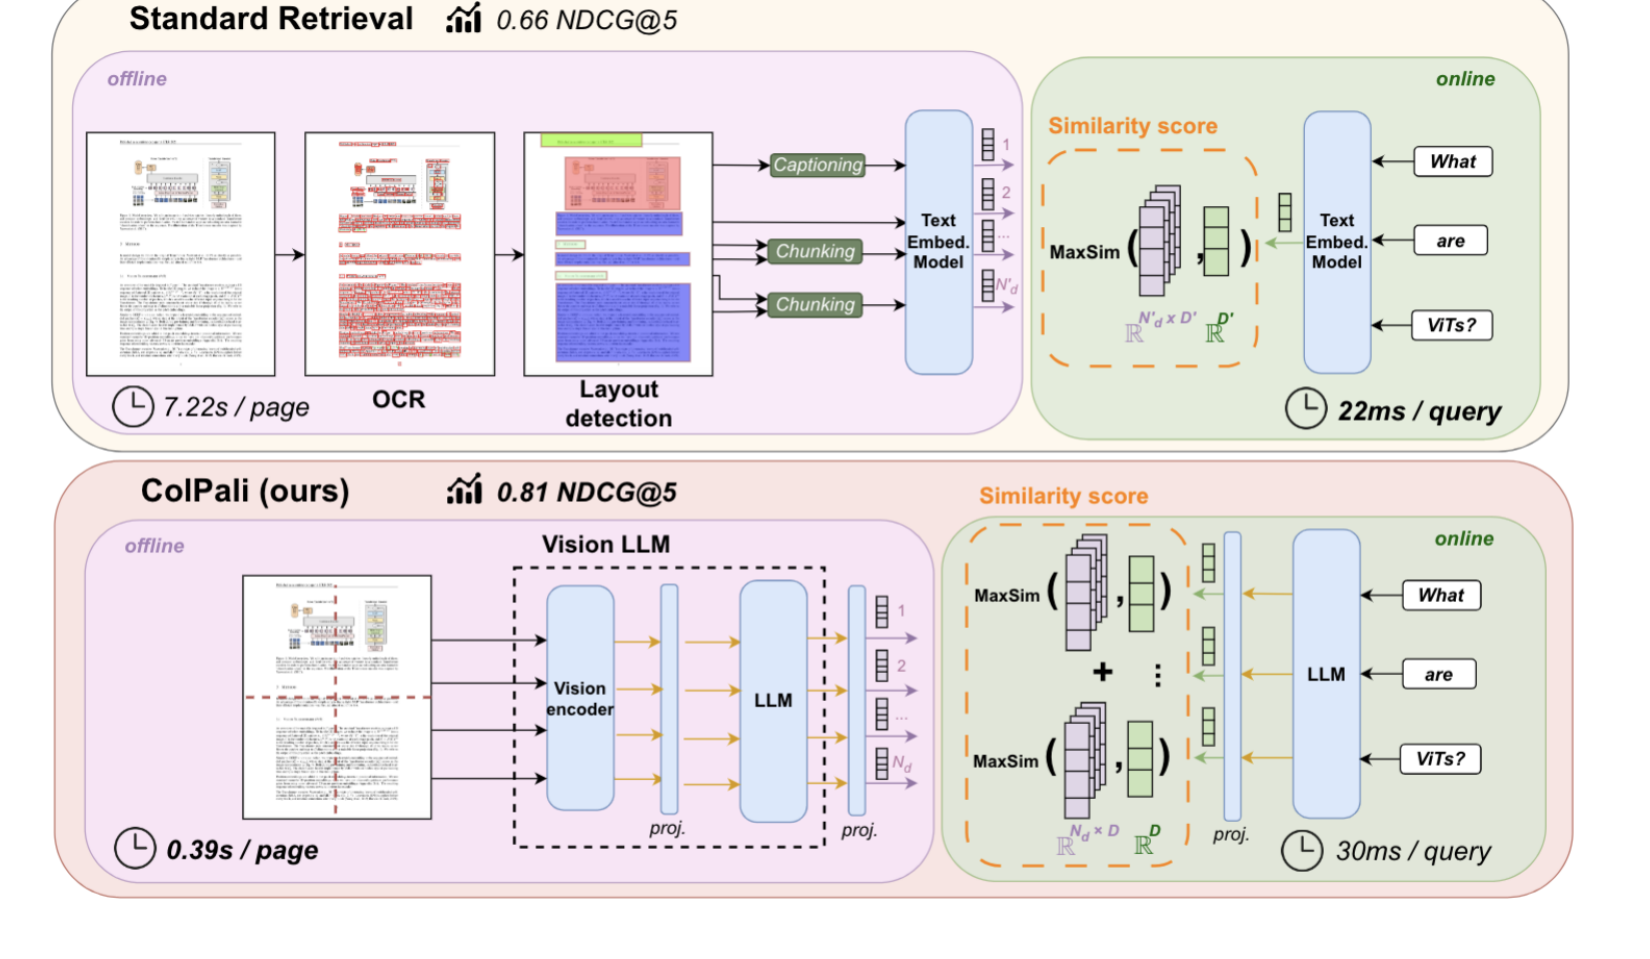
\includegraphics[width=\textwidth]{figures/tv2/colpali-pipeline.png}
    \caption[Quy trình truy xuất truyền thống và ColPali]{Lập chỉ mục và truy vấn ở pipeline truyền thống và ColPali. Nguồn: \cite{faysse2025colpali}.}
    \label{fig:tv2_colpali_pipeline}
\end{figure}

Hình~\ref{fig:tv2_colpali_pipeline} tách bước lập chỉ mục khỏi bước
tìm kiếm. Hệ thống mã hóa ảnh và lập chỉ mục trước khi có câu hỏi.
Khi nhận truy vấn, ColPali nối thêm năm token \texttt{<unused0>} rồi
mới mã hóa. Các token này giúp mô hình học cách mở rộng hoặc điều
chỉnh trọng số của truy vấn. Khi thêm trang mà vẫn dùng cùng mô hình
và quy tắc kết xuất, chỉ cần mã hóa phần mới. Nếu đổi checkpoint hoặc
độ phân giải, cần theo dõi phiên bản embedding để giữ chỉ mục nhất
quán \cite{faysse2025colpali,khattab2020colbert}.

\subsubsection{Toán tử Late Interaction (MaxSim) và hàm mất mát}

Với $\mathbf{q}_i$ là vector của token truy vấn thứ $i$ và $\mathbf{d}_j$
là vector thứ $j$ của trang, ColPali tính điểm theo cơ chế kế thừa từ
ColBERT \cite{khattab2020colbert,faysse2025colpali}
\begin{equation}
    \mathrm{LI}(q,d)
    = \sum_{i=1}^{N_q}\max_{1\le j\le N_d}
        \langle \mathbf{q}_i,\mathbf{d}_j\rangle.
\end{equation}
Mỗi token truy vấn đóng góp thông qua token trang khớp nhất. Do đó,
các từ khác nhau trong câu hỏi có thể khớp với các vùng ảnh khác nhau
trên cùng một trang.


\begin{examplebox}{Minh họa cách tính MaxSim}
Hai token truy vấn có điểm tương đồng với ba vùng của trang A lần lượt
là $(0{,}83,0{,}12,0{,}24)$ và $(0{,}28,0{,}66,0{,}34)$.
Điểm MaxSim của A là $0{,}83+0{,}66=1{,}49$. Trang B có một vùng
khớp token đầu ở mức $0{,}91$, nhưng token sau đạt tối đa $0{,}30$.
Điểm của B là $1{,}21$, nên A xếp trên B. Đây là ví dụ minh họa.
\end{examplebox}

Các token có thể khớp tại những vùng rời nhau. Tên một công ty có
thể nằm ở phần văn bản trong khi tỷ lệ tăng trưởng trên cùng trang
thuộc công ty khác. Điểm MaxSim cao giúp ưu tiên kiểm tra trang.
Bộ đọc còn phải xác minh số liệu thực sự gắn với công ty được hỏi.
Mỗi cặp truy vấn--trang cần $N_qN_d$ tích vô hướng trên vector $D$
chiều nếu chấm trực tiếp. Càng nhiều token hoặc ứng viên, MaxSim
càng phải tính nhiều. Khi đo trên kho lớn, cần ghi rõ số ứng viên
được chấm và cách nén vector.

\paragraph{Hard negatives trong ColPali.}
Với một batch gồm $B$ cặp $(q_i,d_i)$, ColPali dùng các trang của
những truy vấn khác làm in-batch negatives. Gọi $s_i^+$ là điểm của
trang liên quan và $s_i^-$ là điểm của negative được xếp cao nhất.
Hàm mất mát so sánh hai điểm như sau.
\begin{equation}
    \mathcal{L}_{\mathrm{ColPali}} =
    \frac{1}{B}\sum_{i=1}^{B}\log\bigl(1+\exp(s_i^- - s_i^+)\bigr).
    \label{eq:tv2_colpali_loss}
\end{equation}
Khi hard negative xếp trên trang liên quan, hiệu $s_i^- - s_i^+$
và mức phạt tăng. Nếu negative chứa một bản sao của cùng bảng, mô hình
có thể nhận tín hiệu phạt dù trang đó hữu ích. Cần xem xét
chất lượng nhãn khi áp dụng chiến lược này vào kho nhiều phiên bản
tài liệu.

Tập huấn luyện của ColPali chứa 118\,695 cặp truy vấn--trang. Khoảng
63\% đến từ dữ liệu học thuật công khai và 37\% là cặp tổng hợp từ
PDF. Nhóm tác giả dùng truy vấn tiếng Anh và kiểm tra để cùng một PDF
nhiều trang không xuất hiện trong cả tập huấn luyện lẫn tập đánh giá. Cấu hình tham chiếu
huấn luyện 1 epoch với LoRA ($r=32$, $\alpha=32$) ở phần ngôn ngữ,
cùng lớp chiếu mới khởi tạo. Bộ mã hóa ảnh được mở khóa trong một
thí nghiệm khác, xem kết quả ở Mục~\ref{subsec:tv2_ablation}
\cite{faysse2025colpali}.

\subsubsection{Đọc similarity heatmap của truy vấn}

Các điểm $\langle\mathbf{q}_i,\mathbf{d}_j\rangle$ của một token có
thể được đặt trở lại lưới ảnh. Hình~\ref{fig:tv2_colpali_heatmap}
cho thấy token \textit{hour} có điểm tương đồng nổi bật tại chữ
\textit{Hourly} và vùng trục hoành ghi giờ. Với ví dụ khác trong
phụ lục ColPali, từ khóa Kazakhstan còn kích hoạt vùng ghi
Kashagan, một mỏ dầu ở Kazakhstan \cite{faysse2025colpali}.

\begin{figure}[htbp]
    \centering
    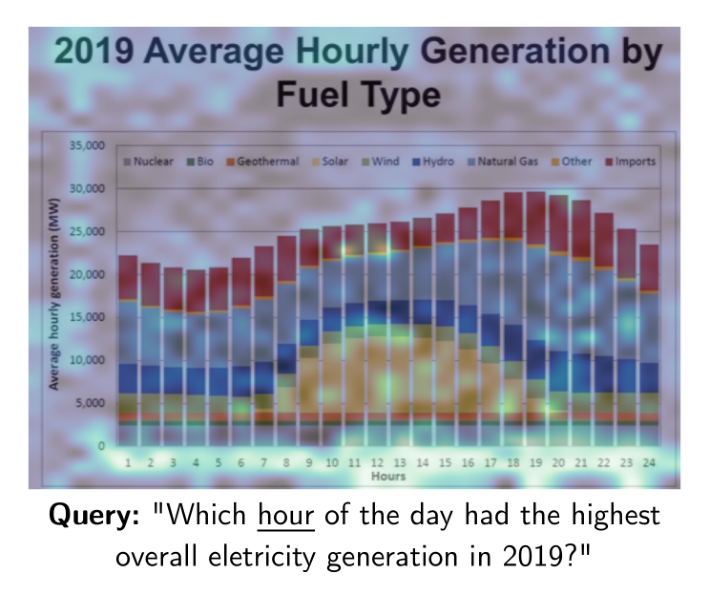
\includegraphics[width=0.72\textwidth]{figures/tv2/colpali-heatmap.png}
    \caption[Bản đồ tương đồng của token hour]{Tương đồng theo mảnh ảnh đối với token \textit{hour}. Nguồn: \cite{faysse2025colpali}.}
    \label{fig:tv2_colpali_heatmap}
\end{figure}

Các vùng sáng giải thích phần nào lý do trang nhận điểm truy xuất cao. Muốn trả lời giờ có tổng sản lượng lớn nhất, bộ đọc còn cần tìm cột cao nhất, xác định đúng số giờ trên trục và đọc phạm vi của biểu đồ. Heatmap hữu ích để kiểm tra chứng cứ mà retriever ưu tiên. Cần đối chiếu riêng nội dung trả lời do bộ sinh đưa ra.

\subsection{VisRAG với Single-vector Embeddings và End-to-End RAG}
\label{subsec:visrag}

\subsubsection{Bộ truy xuất VisRAG-Ret và Position-weighted Mean Pooling}

VisRAG-Ret dùng MiniCPM-V 2.0 để mã hóa câu hỏi và ảnh trang. Cho chuỗi
trạng thái ẩn $\mathbf{h}_1,\ldots,\mathbf{h}_n$, bộ truy xuất gộp chúng
thành một vector với trọng số tăng theo vị trí
\begin{equation}
    \mathbf{e}=\sum_{i=1}^{n}\frac{i}{\sum_{j=1}^{n}j}\,\mathbf{h}_i.
\end{equation}
Các token ở cuối chuỗi có thể tiếp nhận nhiều ngữ cảnh trước đó hơn
nhờ cơ chế causal attention. Điểm truy xuất là cosine similarity
giữa vector truy vấn và vector trang \cite{yu2025visrag}.


Với bốn vị trí, trọng số gộp lần lượt là $0{,}1$, $0{,}2$, $0{,}3$
và $0{,}4$. Hệ thống thu được một vector 2304 chiều cho mỗi trang.
Khi hai vector đã chuẩn hóa theo chuẩn Euclid, cosine tương đương
tích vô hướng. Chỉ mục vector có thể dùng Approximate Nearest
Neighbor (ANN) search. Đổi tham số tìm kiếm có thể giảm độ trễ nhưng cũng
loại trang liên quan khỏi danh sách ứng viên. Vì thế cần đo tỷ lệ
giữ lại trang đúng khi đánh giá tốc độ ở quy mô lớn.

Với truy vấn $q_i$, tập $D_i^-$ gồm các in-batch negatives,
còn $d_i^+$ là trang liên quan. InfoNCE có dạng
\begin{equation}
    \ell_i=-\log
    \frac{\exp(s(q_i,d_i^+)/\tau)}
    {\exp(s(q_i,d_i^+)/\tau)+
      \sum_{d\in D_i^-}\exp(s(q_i,d)/\tau)}.
    \label{eq:tv2_visrag_loss}
\end{equation}
Các negative có điểm cao đóng góp nhiều hơn trong mẫu số.
VisRAG huấn luyện 1 epoch với batch size 128 và $\tau=0{,}02$. Dữ liệu
kết hợp sáu tập hỏi đáp trực quan với các cặp tổng hợp từ giáo
trình, bài báo và tài liệu hướng dẫn. Một câu như “màu đường
thứ hai trong hình này là gì?” có thể được trả lời khi trang đã
cho sẵn, nhưng từ “hình này” ít giá trị trong tìm kiếm độc lập.
Bộ lọc loại các câu phụ thuộc mạnh vào trang cho trước để xây
dựng cặp phù hợp hơn cho huấn luyện truy xuất \cite{yu2025visrag}.

\subsubsection{Bộ tạo sinh VisRAG-Gen cho ngữ cảnh đa trang}
VisRAG-Gen khảo sát ba cách sử dụng các trang đã truy xuất. Với VLM
chỉ nhận một ảnh, hệ thống có thể ghép nhiều trang thành một ảnh
hoặc tạo câu trả lời riêng cho từng trang rồi chọn theo điểm kết hợp
độ tin cậy của bộ sinh với mức liên quan của trang. Với VLM hỗ trợ
nhiều ảnh, hệ thống đưa các trang riêng vào cùng một lượt suy luận
\cite{yu2025visrag}.

Hình~\ref{fig:tv2_visrag_pipeline} minh họa câu hỏi về sự thay đổi độ nhạy tần số từ đáy đến đỉnh ốc tai. Văn bản trích xuất chứa nhiều giá trị Hz rời rạc. Sơ đồ gốc giữ vị trí của từng nhãn số tương ứng cấu trúc giải phẫu, cho phép đọc được xu hướng giảm dần. Ví dụ cho thấy phần lớn ký tự vẫn có thể xuất hiện trong văn bản mà chứng cứ cần cho câu hỏi đã bị mất một phần \cite{yu2025visrag}.

\begin{figure}[htbp]
    \centering
    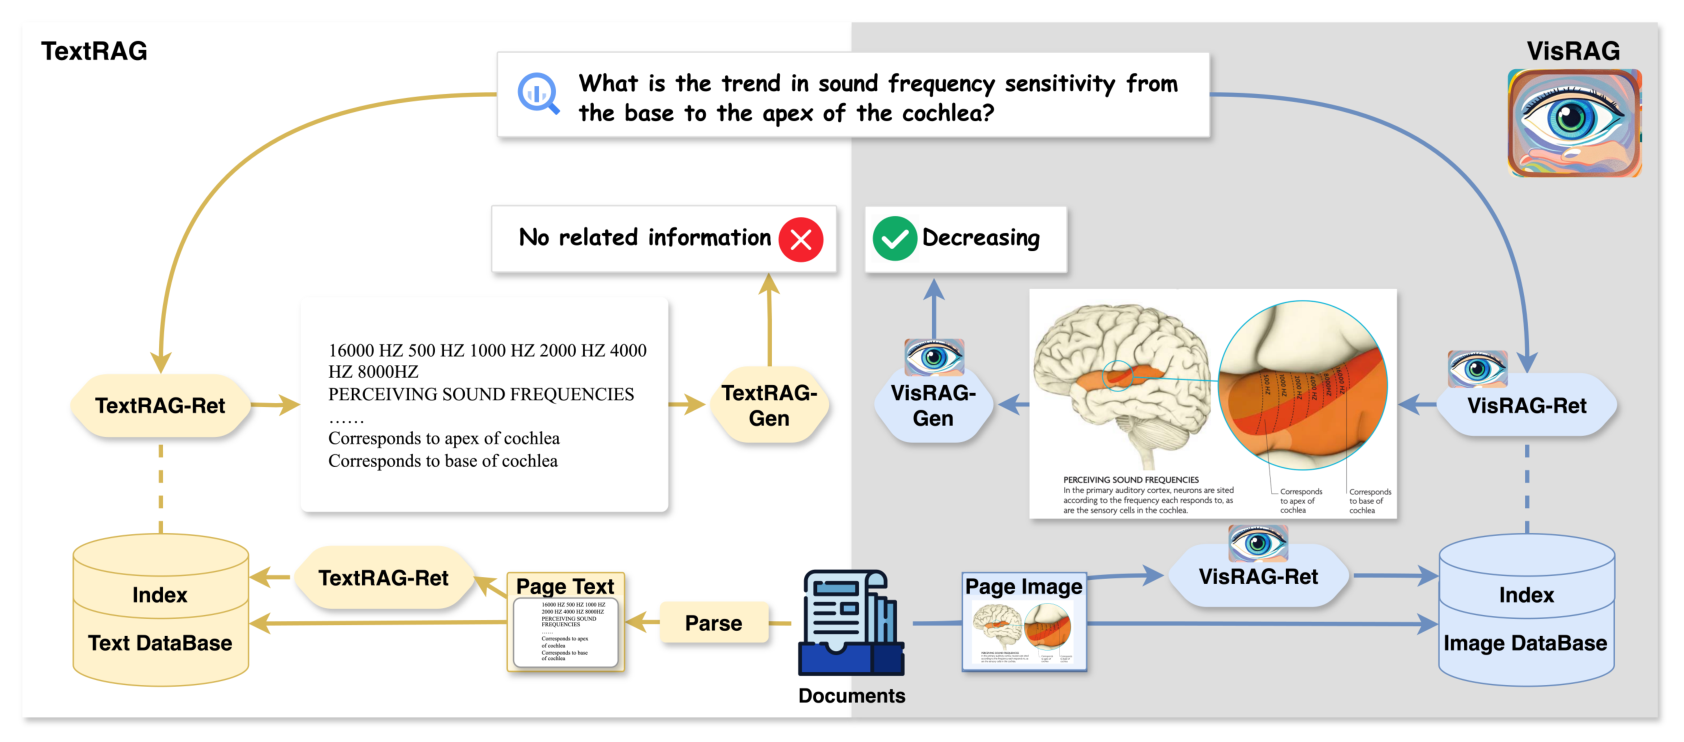
\includegraphics[width=\textwidth]{figures/tv2/visrag-pipeline.png}
    \caption[Luồng xử lý của TextRAG và VisRAG]{Luồng xử lý của TextRAG và VisRAG trong ví dụ sơ đồ ốc tai. Nguồn: \cite{yu2025visrag}.}
    \label{fig:tv2_visrag_pipeline}
\end{figure}

\paragraph{Page Concatenation.}
Các trang được ghép ngang thành một ảnh. MiniCPM-V~2.0 đọc ảnh ghép trong một lượt. Nếu ảnh ghép phải thu nhỏ, chữ nhỏ và các ô ở sát nhau khó phân biệt hơn. Cấu hình ghép còn đặt các trang liền kề dù chúng có thể nằm ở những phần khác nhau của tài liệu.

\paragraph{Weighted Selection.}
Mô hình tạo câu trả lời $a_d$ từ từng trang, sau đó chọn
theo điểm
\begin{equation}
    S(a_d,q,d)=g(a_d\mid q,d)
        \frac{\exp(s(q,d))}
        {\sum_{d'\in\mathcal{D}_{k}}\exp(s(q,d'))},
    \label{eq:tv2_visrag_selection}
\end{equation}
trong đó $\mathcal{D}_{k}$ là tập trang đã truy xuất và $g$ là độ
tin cậy tạo sinh, được tính bằng nghịch đảo perplexity trong bài
gốc. Mỗi câu trả lời ứng viên chỉ dùng một trang. Cấu hình này có
thể chọn được trang hữu ích khi thông tin nằm gọn trên một ảnh.
Nếu câu hỏi cần lấy số liệu từ hai trang, hai câu trả lời riêng
có thể đều thiếu một phần chứng cứ \cite{yu2025visrag}.

\paragraph{Multi-image VLM.}
MiniCPM-V 2.6 và GPT-4o có thể nhận từng ảnh trong cùng một lượt.
Ví dụ, một trang chứa bảng doanh thu và trang kế tiếp ghi đơn
vị quy đổi. Đưa cả hai ảnh vào cho phép đối chiếu giá trị với đơn
vị trước khi tính. Số ảnh tăng cũng làm tăng số token thị giác,
độ trễ và khả năng có trang nhiễu. Thực nghiệm ở
Mục~\ref{subsec:tv2_generation} phân tích kết quả theo số trang
và theo năng lực xử lý ảnh của từng bộ sinh.

\subsubsection{Hai loại lỗi quan sát trên bài kiểm thử}

Trong ví dụ Club Jetty ở Bảng 8 của VisRAG, OCR đọc sai tên nhà
hàng do chữ cách điệu. TextRAG lấy nhầm trang Smokers Express.
VisRAG trả đúng trang \textit{Explore Kauai}, nơi ô quảng cáo ghi
nhà hàng đóng cửa thứ Ba. Đây là lỗi truy xuất. Khi cửa hàng cần
hỏi không xuất hiện trong ngữ cảnh, tăng năng lực bộ sinh khó
khôi phục chứng cứ bị thiếu \cite{yu2025visrag}.

Trong ví dụ LinkedIn ở Bảng 9, cả hai cấu hình đều tìm đúng
infographic. TextRAG trả 49\%, tỷ lệ của Bắc Mỹ, dù truy vấn hỏi
về châu Âu. VisRAG đọc đúng 53\% từ vị trí của nhãn châu Âu.
Lỗi xảy ra sau khi đã tìm đúng trang, ở bước chuẩn bị hoặc đọc
ngữ cảnh. Cả hai phương án đều tìm đúng trang ở hạng đầu nên có cùng
Recall@1 cho câu hỏi này, dù đáp án khác nhau \cite{yu2025visrag}.

\subsection{So sánh đối chứng chuyên sâu: ColPali và VisRAG}
\label{subsec:colpali_vs_visrag}


\begin{table}[H]
\centering
\small
\caption[Bảng đối chứng cơ chế kỹ thuật giữa ColPali và VisRAG]{Bảng đối chứng cơ chế kỹ thuật và đánh đổi thiết kế giữa ColPali và VisRAG.}
\label{tab:colpali_vs_visrag}
\renewcommand{\arraystretch}{1.24}
\begin{tabularx}{\textwidth}{@{}P{3.4cm}L L@{}}
\toprule
\rowcolor{tblhead}
\thead{Tiêu chí đối chiếu} & \thead{ColPali} & \thead{VisRAG} \\
\midrule
Backbone nền tảng & PaliGemma-3B & MiniCPM-V 2.0 (bộ truy xuất) \\
\rowcolor{zebrabg}
Kiểu biểu diễn \& Dung lượng & 1030 vector 128 chiều, khoảng 257,5\,KB/trang & Một vector 2304 chiều, khoảng 4,5\,KB/trang \\
Cơ chế so khớp & Tổng MaxSim theo token & Cosine giữa hai vector gộp \\
\rowcolor{zebrabg}
Khả năng giải thích & Có thể minh họa vùng ảnh khớp với token & Điểm tương đồng ở mức toàn trang \\
Phạm vi giải quyết & Xếp hạng trang & Xếp hạng trang và tạo câu trả lời \\
\rowcolor{zebrabg}
Dữ liệu \& Huấn luyện & Cặp truy vấn--trang, mẫu âm trong batch & Dữ liệu VQA và cặp tổng hợp, mẫu âm trong batch \\
Điểm yếu / Đánh đổi chính & Chỉ mục lớn, nhiều phép so khớp khi chấm điểm & Gộp tín hiệu toàn trang vào một vector \\
\bottomrule
\end{tabularx}
\end{table}

Dung lượng trong Bảng~\ref{tab:colpali_vs_visrag} là kích thước biểu
diễn trang tương ứng với cấu hình của từng bài \cite{faysse2025colpali,yu2025visrag}. Biểu diễn
đa vector giữ tín hiệu ở nhiều vùng của trang. Biểu diễn đơn vector
cần ít bộ nhớ hơn và chấm điểm bằng cosine similarity.

Với hai byte cho mỗi giá trị, ColPali cần
$1030\times128\times2=263\,680$ byte mỗi trang, tương đương
257,5\,KiB. Vector 2304 chiều cần 4608 byte, tức 4,5\,KiB.
Bảng giữ ký hiệu KB theo hai nghiên cứu. Chênh lệch khoảng
57,2 lần áp dụng cho biểu diễn chưa nén. Với một triệu trang,
hai mức này lần lượt xấp xỉ 245,6\,GiB và 4,3\,GiB trước khi
tính cấu trúc chỉ mục, metadata, ảnh tài liệu và bộ nhớ mô hình.
Các lựa chọn độ chính xác lưu trữ khác làm thay đổi dự toán
\cite{faysse2025colpali,yu2025visrag}.

Trên kho báo cáo dày chữ, cần kiểm tra khả năng giữ đúng trang
có bảng và khả năng nén chỉ mục mà không mất vùng chữ nhỏ. Trên
kho lớn và đa dạng, chỉ mục vector đơn thuận tiện để thử tìm kiếm
ứng viên. Các kết quả theo từng tập ở Mục~\ref{subsec:tv2_visrag_ret_results}
cho thấy thứ hạng của hai phương pháp thay đổi giữa DocVQA, SlideVQA,
InfoVQA và PlotQA. Vì vậy, phép đánh giá nên phản ánh loại câu hỏi
người dùng thường gặp, như tìm mã định danh, đọc bảng hay giải thích
biểu đồ.

Có thể dùng vector đơn chọn $m$ ứng viên rồi dùng MaxSim xếp hạng lại. Khi đó cần lưu thêm vector hoặc mã hóa lại ảnh ứng viên. Recall của top-$m$ là giới hạn của bước xếp hạng lại. Mục~\ref{subsec:tv2_protocol} đề xuất cách đo khi kết hợp hai tầng.